\subsection{Experimental Setup}
\label{sec:setup}

\subsubsection{System used}

Experiments are performed on a system featuring an AMD EPYC-7742 processor with $64$ cores, operating at a frequency of $2.25$ GHz. Each core is equipped with a $4$ MB L1 cache, a $32$ MB L2 cache, and shares a $256$ MB L3 cache. The server is set up with $512$ GB of DDR4 system memory and runs Ubuntu $20.04$.


\subsubsection{Configuration}

We use 32-bit integers for vertex IDs and 64-bit floating-point numbers for vertex ranks. Affected vertices are represented with an 8-bit integer vector. Rank computation employs OpenMP's \textit{dynamic schedule} with a chunk size of $2048$ for dynamic workload balancing among threads. We set the damping factor to $\alpha = 0.85$ \cite{rank-langville06} and an iteration tolerance of $\tau = 10^{-10}$ using the $L_\infty$-norm \cite{rank-dubey22, rank-plimpton11}. The maximum number of iterations $MAX\_ITERATIONS$ is limited to $500$ \cite{nvgraph}. All experiments run with $64$ threads to match the available system cores, unless stated otherwise. Compilation is done using GCC $9.4$ and OpenMP $5.0$.


\subsubsection{Dataset}
\label{sec:dataset}

We utilize five temporal networks from the Stanford Large Network Dataset Collection \cite{snapnets}, outlined in Table \ref{tab:dataset}. These networks contain vertex counts ranging from $24.8$ thousand to $2.60$ million, temporal edge counts from $507$ thousand to $63.4$ million, and static edge counts from $240$ thousand to $36.2$ million. To address dead ends (vertices lacking out-links), a global teleport rank computation is needed in each iteration. We mitigate this overhead by adding self-loops to all vertices\ignore{ in the graph} \cite{kolda2009generalized, rank-andersen07, rank-langville06}.

\begin{table}[hbtp]
  \centering
  \caption{List of 5 real-world dynamic graphs\ignore{, i.e., temporal networks}, obtained from the Stanford Large Network Dataset Collection \cite{snapnets}. Here, $|V|$ is the number of vertices, $|E_T|$ the number of temporal edges\ignore{(includes duplicate edges)}, and $|E|$ the number of static edges (with no duplicates).\ignore{, and $\Gamma_G$ is the Gini coefficient of PageRank distribution. In the table, B refers to a billion, M refers to a million and K refers a thousand.}}
  \label{tab:dataset}
  \begin{tabular}{|c||c|c|c|c|}
    \toprule
    \textbf{Graph} &
    \textbf{\textbf{$|V|$}} &
    \textbf{\textbf{$|E_T|$}} &
    \textbf{\textbf{$|E|$}} \\
    \midrule
    sx-mathoverflow & 24.8K & 507K & 240K \\ \hline
    sx-askubuntu & 159K & 964K & 597K \\ \hline
    sx-superuser & 194K & 1.44M & 925K \\ \hline
    wiki-talk-temporal & 1.14M & 7.83M & 3.31M \\ \hline
    sx-stackoverflow & 2.60M & 63.4M & 36.2M \\ \hline
  \bottomrule
  \end{tabular}
\end{table}



\subsubsection{Batch Generation}
\label{sec:batch-generation}

In each experiment, we initially load $90\%$ of every real-world dynamic graph from Table \ref{tab:dataset}, followed by loading $B$ edges consecutively in $100$ batch updates. Here, $B$ represents the desired batch size, specified as a fraction of the total number of temporal edges $|E_T|$ in the graph. Additionally, self-loops are added to all vertices with each batch update.


\subsubsection{Measurement}
\label{sec:measurement}

We evaluate the runtime of each approach on the entire updated graph, including preprocessing and convergence detection time, but excluding memory allocation/deallocation time. The mean time and error for a specific method at a given batch size is computed as the geometric mean across input graphs.\ignore{Average speedup is the ratio of these mean times.} Additionally, we assess the error/accuracy of each approach by measuring the $L1$-norm \cite{ohsaka2015efficient} of the ranks compared to ranks obtained from a reference Static PageRank run on the updated graph with an extremely low iteration tolerance of $\tau = 10^{-100}$ (limited to $500$ iterations).




\subsection{Performance comparison}

\subsubsection{Results on real-world dynamic graphs}

We now compare the performance of our improved Dynamic Frontier (DF) and Dynamic Frontier with Pruning (DF-P) PageRank algorithms with Static, Naive-dynamic (ND), and Dynamic Traversal (DT) PageRank on real-world dynamic graphs from Table \ref{tab:dataset}. This is done on batch updates of size $10^{-5}|E_T|$ to $10^{-3}|E_T|$ in multiples of $10$. For each batch size, we load $90\%$ of the graph initially and then load $B$ edges (where $B$ is the batch size) consecutively in $100$ batch updates. Self-loops are added to all vertices with each batch update. Figure \ref{fig:temporal-summary--runtime-overall} displays the overall runtime of each approach across all graphs for each batch size, while Figure \ref{fig:temporal-summary--error-overall} illustrates the overall rank error compared to a reference Static PageRank run (as described in Section \ref{sec:measurement}). Additionally, Figures \ref{fig:temporal-summary--runtime-graph} and \ref{fig:temporal-summary--error-graph} present the mean runtime and rank error of the approaches on each dynamic graph in the dataset. Finally, Figures \ref{fig:temporal-sx-mathoverflow}, \ref{fig:temporal-sx-askubuntu}, \ref{fig:temporal-sx-superuser}, \ref{fig:temporal-wiki-talk-temporal}, and \ref{fig:temporal-sx-stackoverflow} show the runtime and rank error of the approaches on each dynamic graph in Table \ref{tab:dataset}, upon each consecutive batch update.

Figure \ref{fig:temporal-summary--runtime-overall} shows that DF PageRank is, on average, $8.0\times$, $4.5\times$, and $3.2\times$ faster than Static PageRank for batch updates of size $10^{-5}|E_T|$, $10^{-4}|E_T|$, and $10^{-3}|E_T|$ respectively. Further, DF PageRank is, on average, $1.3\times$, $1.1\times$, and $1.5\times$ faster than DT PageRank, a widely used approach for updating PageRank on dynamic graphs, on the same batch updates. In contrast, DF-P PageRank is, on average, $26.2\times$, $11.9\times$, and $7.5\times$ faster than Static PageRank for batch updates of size $10^{-5}|E_T|$, $10^{-4}|E_T|$, and $10^{-3}|E_T|$ respectively. Furthermore, DF-P PageRank is, on average, $4.2\times$, $2.8\times$, and $3.6\times$ faster than DT PageRank on identical batch updates. This speedup is particularly higher on the \textit{sx-askubuntu} dynamic graph, with both DF and DF-P PageRank, as indicated by Figure \ref{fig:temporal-summary--runtime-graph}.

Regarding rank error, Figure \ref{fig:temporal-summary--error-overall} indicates that DF and DF-P PageRank have, on average, higher error than ND and DT PageRank but lower error than Static PageRank. This makes the ranks obtained with DF and DF-P PageRank acceptable. However, the error in ranks obtained with DF-P PageRank is consistently higher than that of Static PageRank on the \textit{sx-mathoverflow} dynamic graph (see Figure \ref{fig:temporal-summary--error-graph}), making DF PageRank the preferred approach on this particular graph. Therefore, DF-P PageRank can be the default choice for updating PageRank scores on dynamic graphs, but if higher error is observed (through intermediate empirical tests), switching to DF PageRank is recommended.


\subsubsection{Results on large graphs with random updates}

We also evaluate the performance of our improved Dynamic Frontier (DF) and Dynamic Frontier with Pruning (DF-P) PageRank algorithms alongside Static, Naive-dynamic (ND), and Dynamic Traversal (DT) PageRank on large (static) graphs from Table \ref{tab:dataset-large}, with randomly generated batch updates. This is done on batch updates of size $10^{-7}|E|$ to $0.1|E|$ (in multiples of $10$), comprising $80\%$ edge insertions and $20\%$ edge deletions in order to simulate realistic batch updates. Edge insertions are generated by selecting vertex pairs with equal probability, while edge deletions involve deleting each existing edge with a uniform probability. No new vertices are added to or removed from the graph, and self-loops are added to all vertices with each batch update. Figure \ref{fig:8020-runtime} illustrates the runtime of Static, ND, DT, DF, and DF-P PageRank, while Figure \ref{fig:8020-error} depicts the error in ranks obtained with each approach.

Figure \ref{fig:8020-runtime--mean} illustrates that for batch updates ranging from $10^{-7}|E|$ to $10^{-3}|E|$, comprising $80\%$ insertions and $20\%$ deletions, DF PageRank is, on average, $7.2\times$, $2.6\times$, and $4.0\times$ faster than Static, ND, and DT PageRank respectively. Additionally, DF-P PageRank is, on average, $9.6\times$, $3.9\times$, and $5.6\times$ faster than Static, ND, and DT PageRank respectively. This speedup is particularly higher on road networks and protein k-mer graphs, which have a low average degree (as depicted in Figure \ref{fig:8020-runtime--all}). It's worth noting that DT PageRank is slower than ND PageRank \cite{sahu2024incrementally} on large (static) graphs with uniformly random batch updates, as it ends up marking a large number of vertices as affected. This is due to updates being randomly scattered across the graph, leading to most of the graph being reachable from the updated regions.

Figure \ref{fig:8020-error--mean} indicates that DF-P PageRank generally exhibits higher error compared to ND, DT, and DF PageRank, but lower error than Static PageRank (up to a batch size of $10^{-2}|E|$). However, Figure \ref{fig:8020-error--all} highlights that the rank error with DF-P PageRank surpasses that of Static PageRank on web graphs. Consequently, DF PageRank is recommended as the preferred approach for web graphs with random batch updates.


\subsubsection{Comparison of vertices marked as affected}

Figure \ref{fig:measure-affected} displays the (mean) percentage of vertices marked as affected by Dynamic Traversal (DT), our improved Dynamic Frontier (DF), and Dynamic Frontier with Pruning (DF-P) PageRank on real-world dynamic graphs from Table \ref{tab:dataset}. This analysis is conducted on batch updates of size $10^{-5}|E_T|$ to $10^{-3}|E_T|$ in multiples of $10$ (see Section \ref{sec:batch-generation} for details). For DF and DF-P PageRank, affected vertices are marked incrementally --- therefore, we count all vertices that were ever flagged as affected.

As Figure \ref{fig:measure-affected} indicates, the proportion of vertices marked as affected by DF and DF-P PageRank is lower than DT PageRank for batch updates of size $10^{-5}|E_T|$, but comparable for larger batch updates. Therefore, the performance improvement with DF and DF-P PageRank is primarily attributed to the incremental marking of affected vertices. Additionally, it's worth noting that the percentage of vertices marked as affected is generally low across all approaches. This is likely because updates in real-world dynamic graphs tend to be concentrated in specific regions of the graph rather than being scattered throughout.

\begin{figure*}[!hbt]
  \centering
  \subfigure[Overall Runtime]{
    \label{fig:temporal-summary--runtime-overall}
    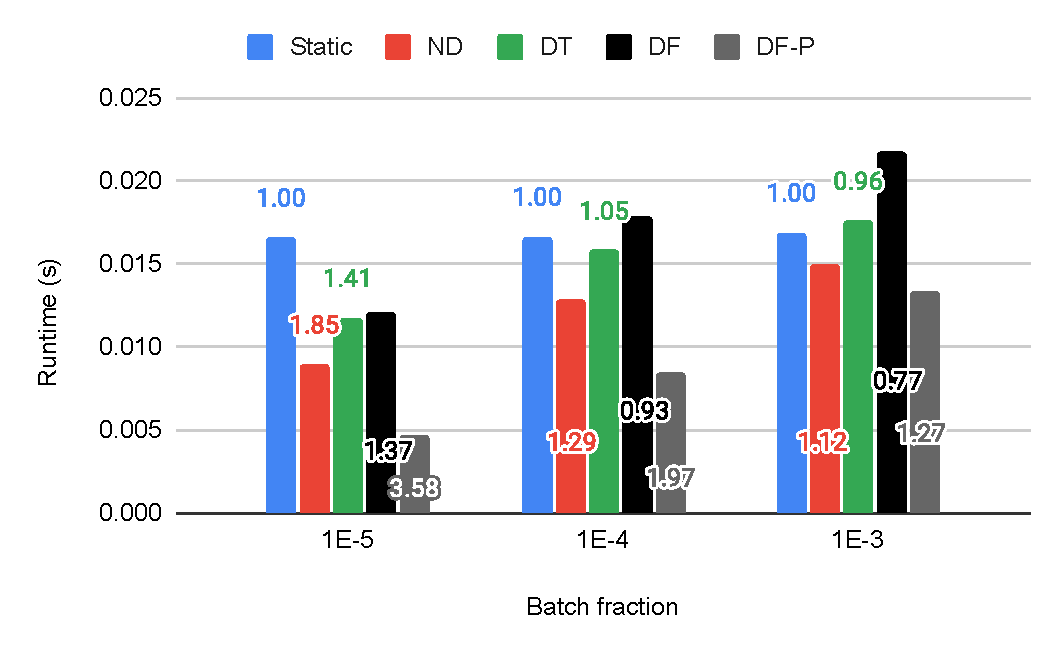
\includegraphics[width=0.48\linewidth]{out/temporal-summary-runtime-overall.pdf}
  }
  \subfigure[Overall Error in ranks obtained]{
    \label{fig:temporal-summary--error-overall}
    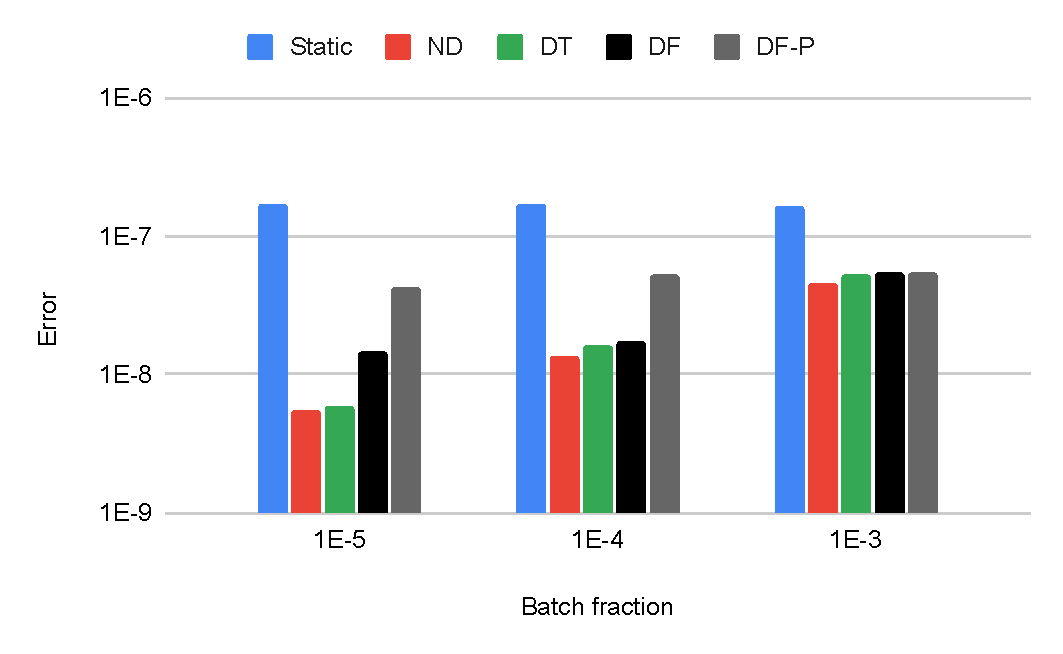
\includegraphics[width=0.48\linewidth]{out/temporal-summary-error-overall.pdf}
  } \\[2ex]
  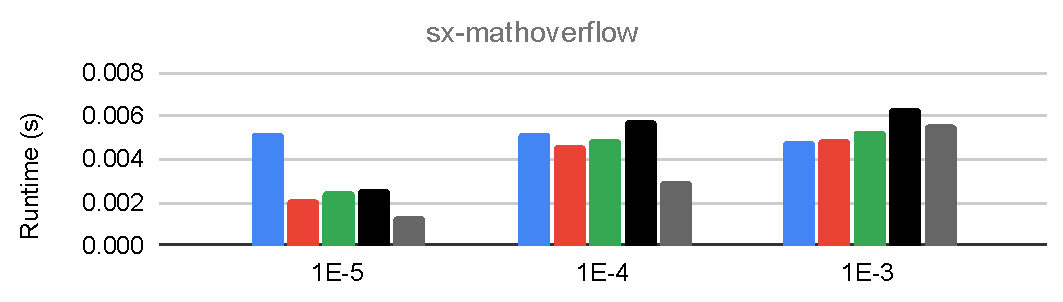
\includegraphics[width=0.48\linewidth]{out/temporal-summary-runtime-sx-mathoverflow.pdf}
  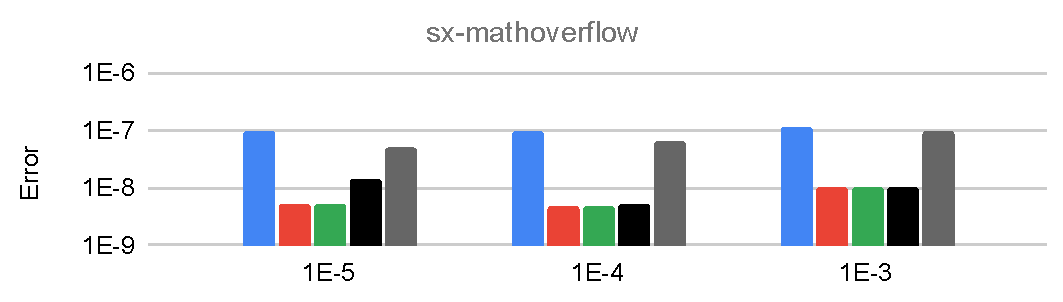
\includegraphics[width=0.48\linewidth]{out/temporal-summary-error-sx-mathoverflow.pdf}
  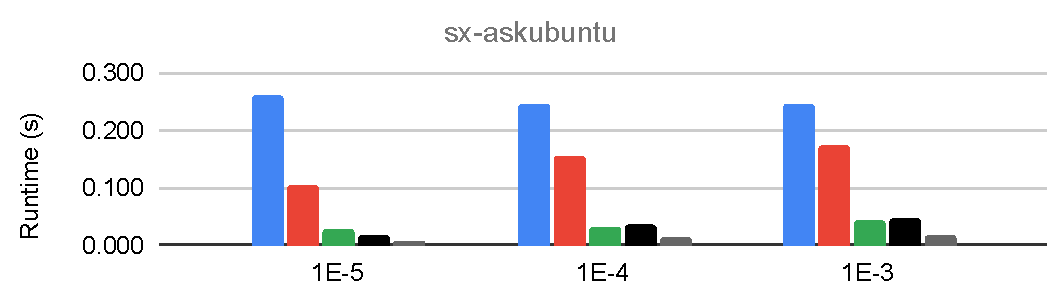
\includegraphics[width=0.48\linewidth]{out/temporal-summary-runtime-sx-askubuntu.pdf}
  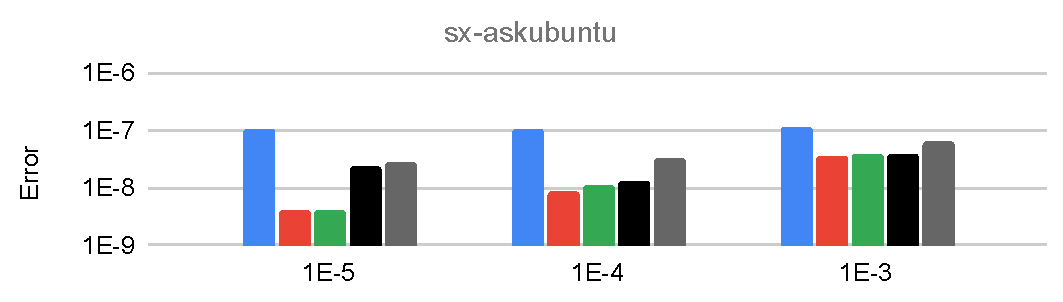
\includegraphics[width=0.48\linewidth]{out/temporal-summary-error-sx-askubuntu.pdf}
  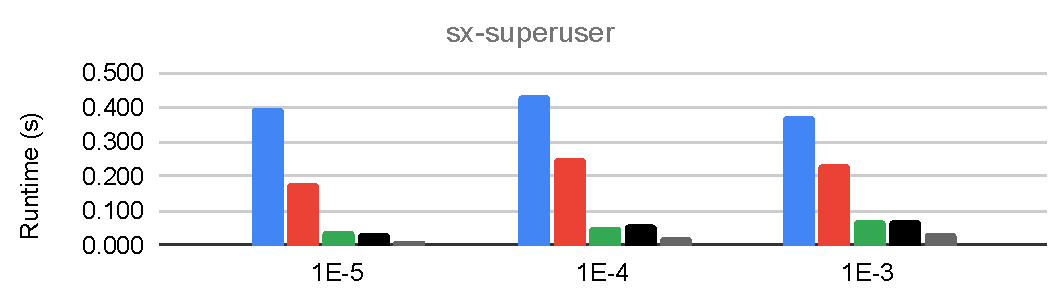
\includegraphics[width=0.48\linewidth]{out/temporal-summary-runtime-sx-superuser.pdf}
  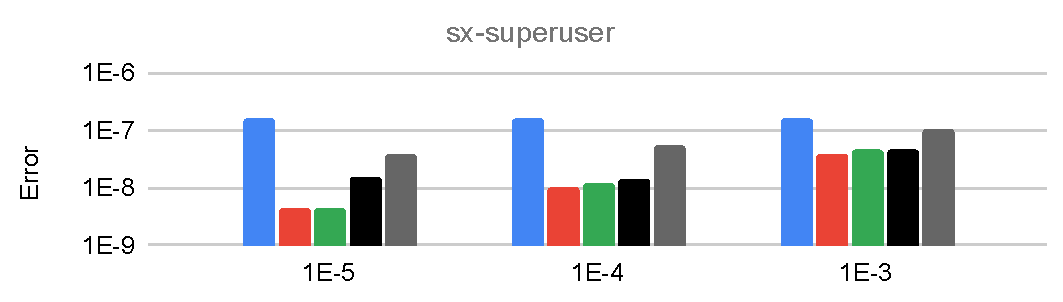
\includegraphics[width=0.48\linewidth]{out/temporal-summary-error-sx-superuser.pdf}
  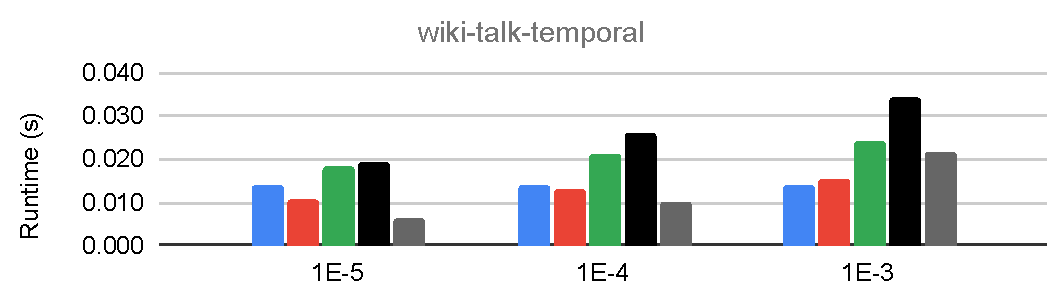
\includegraphics[width=0.48\linewidth]{out/temporal-summary-runtime-wiki-talk-temporal.pdf}
  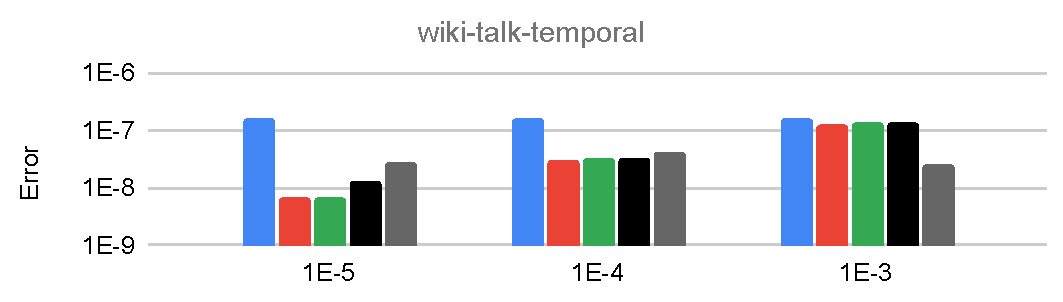
\includegraphics[width=0.48\linewidth]{out/temporal-summary-error-wiki-talk-temporal.pdf}
  \subfigure[Runtime on each dynamic graph]{
    \label{fig:temporal-summary--runtime-graph}
    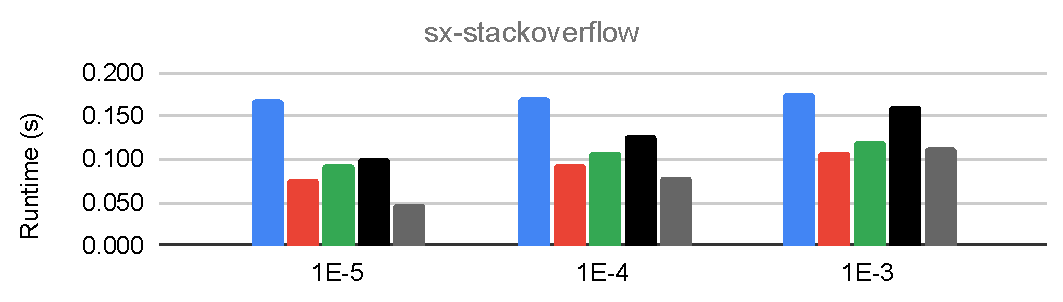
\includegraphics[width=0.48\linewidth]{out/temporal-summary-runtime-sx-stackoverflow.pdf}
  }
  \subfigure[Error in ranks obtained on each dynamic graph]{
    \label{fig:temporal-summary--error-graph}
    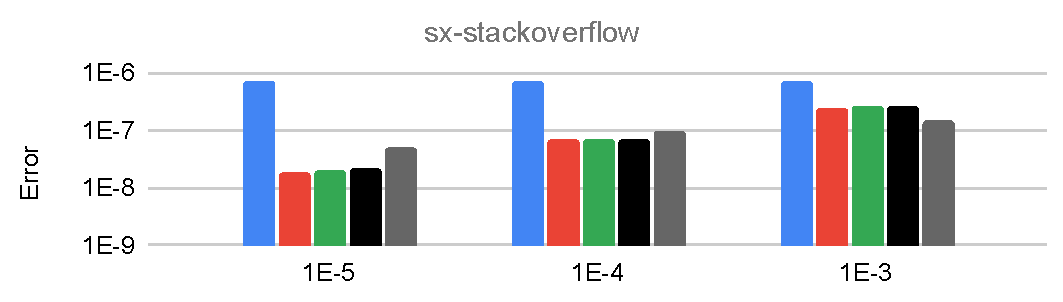
\includegraphics[width=0.48\linewidth]{out/temporal-summary-error-sx-stackoverflow.pdf}
  } \\[-2ex]
  \caption{Mean Runtime and Error in ranks obtained with \textit{Static}, \textit{Naive-dynamic (ND)}, \textit{Dynamic Traversal (DT)}, our improved \textit{Dynamic Frontier (DF)}, and our improved \textit{Dynamic Frontier with Pruning (DF-P)} PageRank on real-world dynamic graphs, with batch updates of size $10^{-5}|E_T|$ to $10^{-3}|E_T|$. Here, (a) and (b) show the overall runtime and error across all temporal graphs, while (c) and (d) show the runtime and rank error for each approach (relative to reference Static PageRank, see Section \ref{sec:measurement}). In (a), the speedup of each approach with respect to Static PageRank is labeled. \su{TOWR}}
  \label{fig:temporal-summary}
\end{figure*}

\begin{figure}[!hbt]
  \centering
  \subfigure{
    \label{fig:measure-affected--batch}
    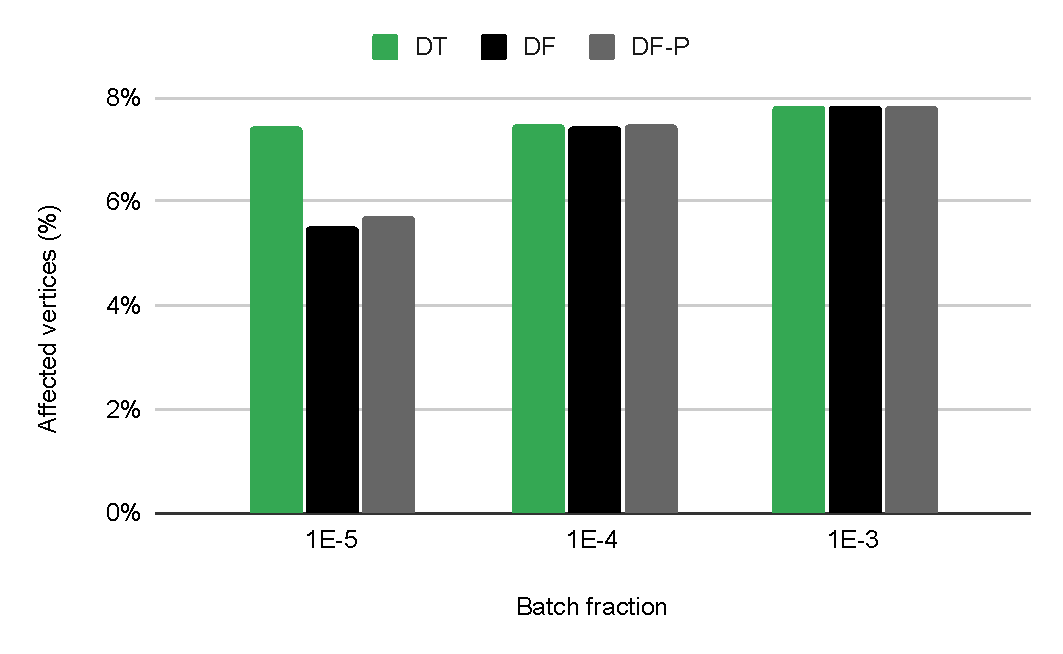
\includegraphics[width=0.98\linewidth]{out/measure-affected-batch.pdf}
  } \\[-2ex]
  \caption{Mean percentage of vertices marked as affected by \textit{Dynamic Traversal (DT)}, our improved \textit{Dynamic Frontier (DF)}, and \textit{Dynamic Frontier with Pruning (DF-P)} PageRank, on real-world graphs, with batch updates of size $10^{-5}|E_T|$ to $10^{-3}|E_T|$ (in multiples of $10$). DF and DF-P PageRank mark affected vertices incrementally --- thus, we count any vertex ever marked as affected. \su{TODO}}
  \label{fig:measure-affected}
\end{figure}

\begin{figure}[!hbt]
  \centering
  \subfigure{
    \label{fig:strong-scaling--speedup}
    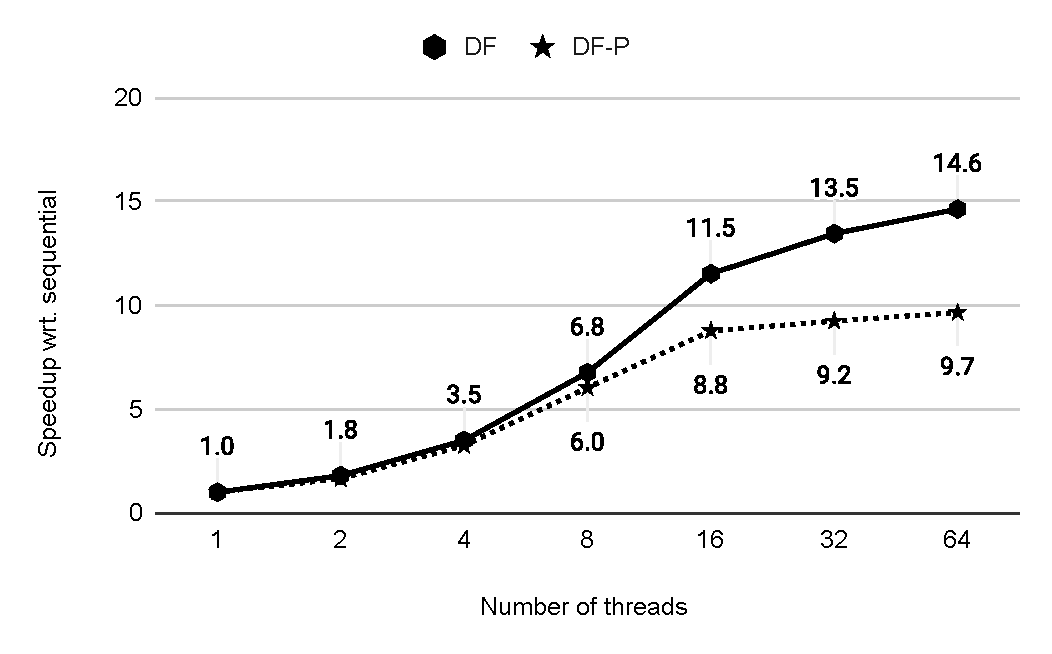
\includegraphics[width=0.98\linewidth]{out/strong-scaling-speedup.pdf}
  } \\[-2ex]
  \caption{Mean speedup of our improved \textit{Dynamic Frontier (DF)} and \textit{Dynamic Frontier with Pruning (DF-P)} PageRank with increasing number of threads (in multiples of $2$), on real-world dynamic graphs, with batch updates of size $10^{-4}|E_T|$.}
  \label{fig:strong-scaling}
\end{figure}





\subsection{Strong Scaling}

Finally, we examine the strong-scaling behavior of our improved Dynamic Frontier (DF) and Dynamic Frontier with Pruning (DF-P) PageRank algorithms on real-world dynamic graphs, with batch updates of a fixed size of $10^{-4}|E_T|$. The speedup of DF and DF-P PageRank is measured as the number of threads increases from $1$ to $64$ in multiples of $2$, relative to single-threaded execution. This process is repeated for each graph in the dataset (refer to Table \ref{tab:dataset}), and the results are averaged using geometric mean.

The results, depicted in Figure \ref{fig:strong-scaling}, indicate that with $16$ threads, DF PageRank achieves an average speedup of $11.5\times$ compared to single-threaded execution, showing a performance increase of $1.8\times$ for every doubling of threads. On the other hand, DF-P PageRank achieves an average speedup of $8.8\times$, suggesting a performance increase of $1.7\times$ for every doubling of threads. The speedup of DF-P PageRank is lower, likely due to the reduced work performed by the algorithm. At $32$ and $64$ threads, both DF and DF-P PageRank are affected by NUMA effects (the $64$-core processor used has $4$ NUMA domains), resulting in a speedup of only $13.5\times$ and $14.6\times$ for DF PageRank, and $9.2\times$ and $9.7\times$ for DF-P PageRank, respectively.
